% Last updated in April 2018 by S. Hamid Rezatofighi
% Based on CVPR 07 and LNCS style, with modifications by DAF, AZ and elle 2008, AA 2010, ACCV 2010

\documentclass[runningheads]{llncs}
\usepackage{graphicx}
\usepackage{amsmath,amssymb} % define this before the line numbering.
\usepackage{ruler}
\usepackage{color}

%===========================================================
\begin{document}
\pagestyle{headings}
\mainmatter

\def\ACCV18SubNumber{***}  % Insert your submission number here

%===========================================================
\title{Convolutional Layer Aggregation using LSTM} % Replace with your title
\titlerunning{ACCV-18 submission ID \ACCV18SubNumber}
\authorrunning{ACCV-18 submission ID \ACCV18SubNumber}

\author{Yu Qin}
\institute{Paper ID \ACCV18SubNumber}

\maketitle

%===========================================================
\begin{abstract}
The abstract should summarize the contents of the paper and should
contain at least 70 and at most 300 words. It should be set in 9-point
font size and should be inset 1.0~cm from the right and left margins.
\dots
\end{abstract}

%===========================================================
\section{Introduction}

In recent years, Convolutional Neural Networks (CNNs) have shown remarkable advantage on computer vision tasks like image classification[]. The basic architecture of convolutional layer consists of two levels, feature extraction and feature mapping. In feature extraction level, the input of each convolutional neuron is connected to local receptive domain and the local characteristics are extracted. Feature mapping level employs multiple convolutional kernels to focus on diferent aspects of the characteristics. The results of each convolutional layer are customarily regarded as features containing spatial and channel-wise information. A series of convolutional layers are stacked together to expand the field of reception and to generate higher level features. The evolution of CNNs from LeNet[] to DenseNet[] increases both the performance and the size of the network, which yields deeper and wider network structures.

From the first application in ResNet[], skip connections have been introduced into CNN structures, and proven effective in various vision tasks. Skip connections combine the output of previous layer and the current layer, dealing with the gradient vanishing problem. DenseNet[] connects densely in a block to make better use of previous features. To further utilize features from different layers, Yu[deep layer aggregation] extends the current skip connection approach proposes deep layer aggregation architectures. These architectures simply combine features of different level by concatenation or addition, without considering the interior relationship between low-level and high-level feature representations. 

Recurrent Neural Networks (RNNs)[] has been proposed to deal with sequantial data like text or speech. Different from feedforward neural networks, RNNs build connections between nodes which are in the same layer. RNNs can be unfolded as a directed graph along the time steps, with all the layers sharing the same weights. This makes RNNs applicable to sequential tasks such as text classification. Long Short Term Memory (LSTM)[] is a special RNN, which makes use of three gates to select valuable information from all the memories. LSTM has proven to be more efficient than normal RNNs in most tasks on sequences.

In this work, we investigate a brand new approach to convolutional layer aggregation, by introducing a new architecture which is named as '\emph{Concolutional Neural Networks-Recurrent Aggregation}' (CNN-RA).  Our goal is to aggregate outputs of multiple layers and retrieve more expressive features. To achieve this, we build CNN-RA by building parallel connection between a CNN and a LSTM. Features from lower Convolutional layers to higher layers naturally form a sequance with a variety of information. This kind of sequence contains both the features themselves and the transformation relationship between different features, which directly leads us to RNNs. We crearte information between outputs of convolutional layers and the inputs of LSTM, and employ the outputs of LSTM as the final feature for tasks such as image classification.

The receptive fields and feature maps sizes of different convolutional layers vary from each other, especially for two layers with a pooling layer inside. We propose an algorithm to transform different shape of feature matrixes to vectors with the same dimention. Then transformed vectors are stacked together as inputs of LSTM. The number of chosen features is the step lengh of the LSTM.

The development of new network architectures is always a time consuming task with abundant hyper parameters to determine. Previous work on layer aggreegation such as DLA[] brings with huge change on the original network architecture, which can even be much more complicated. However, our proposed CNN-RA won't do any modification on the original network, by only connecting it with a parallel LSTM. This property enable CNN-RA easily applicable to multiple convolutional network structures. 

Our evaluation experiments extend famous network structures VGG[] and ResNet[] for standard image classification dataset. The testing results show improvements across different network structures and datasets. The connected LSTM brings with higher performance without increasing much parameter count. The experiment processes show that the relationship between two convolutional blocks with a down sampling layer inside has the most important contribution to the model.

%Do not use any additional Latex macros.

%------------------------------------------------------------------------- 

\section{Related Work}

\section{Methodology}
Convolutional layer aggregation is a combination of features from different layers. The output matrices of convolutional layers are regarded as expressive features for vision tasks. In general, shallow layers contain low-level features and deep layers contain high-level features. Existing work simply uses high-level features or a combination of all layers. In this work, we take into account both feature combination and the sequential tranformation relationship between all levels. Output features of convolutional layers form a sequence and RNNs are born to deal with sequential data. LSTM is employed to do the layer aggregation on CNN in this paper. The output shape of different layers varies, therefore we use mapping nodes to map selected features to the same dimention, and aggregrate them to be the input of LSTM. The structure diagram of CNN-RA is shown in Fig.~\ref{fig:CNN-RA}.

Recent network design tends to assemble serveral blocks together and simplify the network representation. Several layers are grouped into a single block which is capable of realizing some feature extraction and transformation function. Our proposed aggregation method employs the output of blocks instead of all layers to focus on useful but not redundant information.

\begin{figure}  
	\centering
	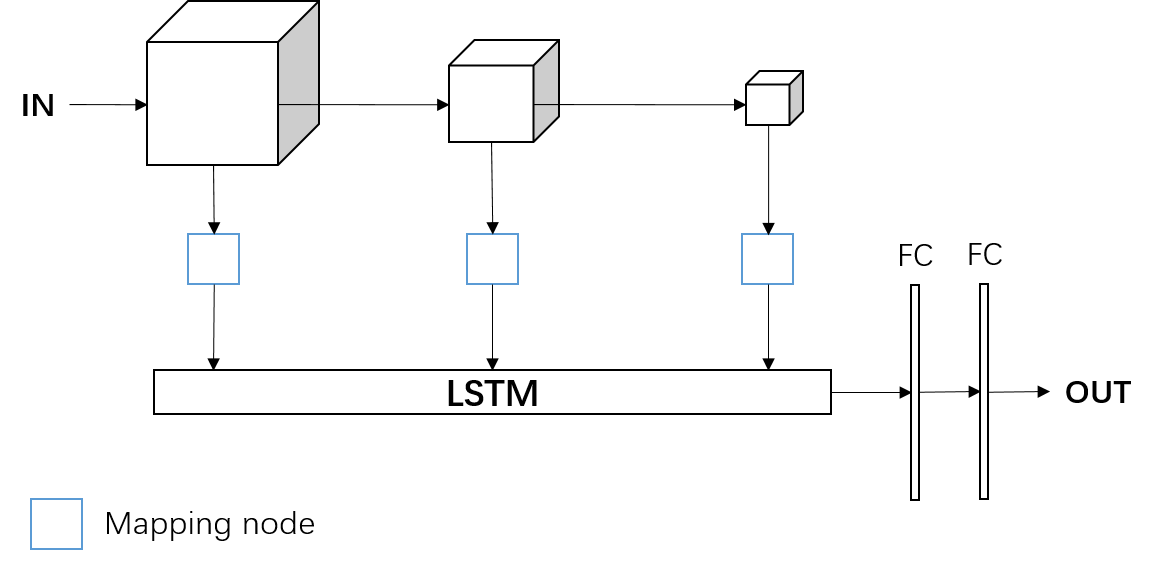
\includegraphics[width=12cm]{Figures/CNN-RA.png}
	\caption{Structure of CNN-RA}
	\label{fig:CNN-RA}
\end{figure}

\subsection{Convolutional Feature Mapping}

Convolutioanl feature mapping helps transform feature matrices of different blocks into vectors with the same dimention. The feature resolution and number of channels varies among blocks because of convolution and down-sampling operations. Then the blocks are grouped into stages according to their output shape. Blocks within the same stage shares common mapping operation which is different from other stages. In general, deeper layer holds smaller feature resolution and more channels. We propose to take the feature matrix of the last block as the standard $S \in \mathbb{R}^{H\times W \times C}$ and transform other matrices towards it. 

The standard $S$ contains high-level features and each unit of $S$ holds a large receptive field size due to previous convolution and down-sampling operations. For such output features we tend to exploit their channel dependencies instead total information. Therefore, we do global average pooling on $S$ to squeeze the spacial information into a channel-wise vector. Then a channel descripter $D\in \mathbb{R}^C$ is generated with the $c_{th}$ element calculated by:
\begin{equation}
D_c = F_{gp}(S_c) = \frac{1}{H\times W}\sum_{i=1}^H\sum_{j=1}^W S_c(i,j).
\end{equation}

Shallow blocks, where each unit can cover a limited region of receptive field, contain local information and this information helps extract fine features. Our propposed layer aggregation pay attention to both low-level and high-level features,  and thus global average pooling operation is not suitable for these shallow blocks. We embed a convolutional layer with kernel size $k\times k$ and stride $l=k$ to combine local information, and then use average pooling layer with kernel size equal to the feature map shape of $S$.  An output matrix $U\in \mathbb{R}^{h\times w\times c}$ is generated with $h\times w\times c=C$.  We then expand the matrix $U$ to a vector with the same length as $D$.

The receptive fields of  blocks in middle stages are large enough to cover the input image, and the numbers of channels are normally less than $C$. For these kinds of blocks, we first embed a convolutional layer with channel number $C$ to ectend the channel number, and then take global average pooling on the output. A vector with length $C$ is then generated.

The generated vectors share the same length and can be arranged into a matrix. Given a network structure with $N$ blocks and then we can generate a feature matrix $V\in \mathbb{R}^{N\times C}$.

\subsection{Recurrent Aggregation using LSTM}
After convolutional feature mapping we get a matrix $V\in \mathbb{R}^{N\times C}$. The matrix is constructed by assembling a sequence of $N$ feature vectors $v \in \mathbb{R}^{1\times C}$ and we denote $V=[v_1, v_2, \cdots, v_N]$. As shown in Fig.~\ref{fig:CNN-RA}, the sequential vectors are arranged according to the generated order in the CNN structure, and $[v_1$ to $v_N]$ denote from low-level feature to high-level feature. 
\begin{figure}  
	\centering
	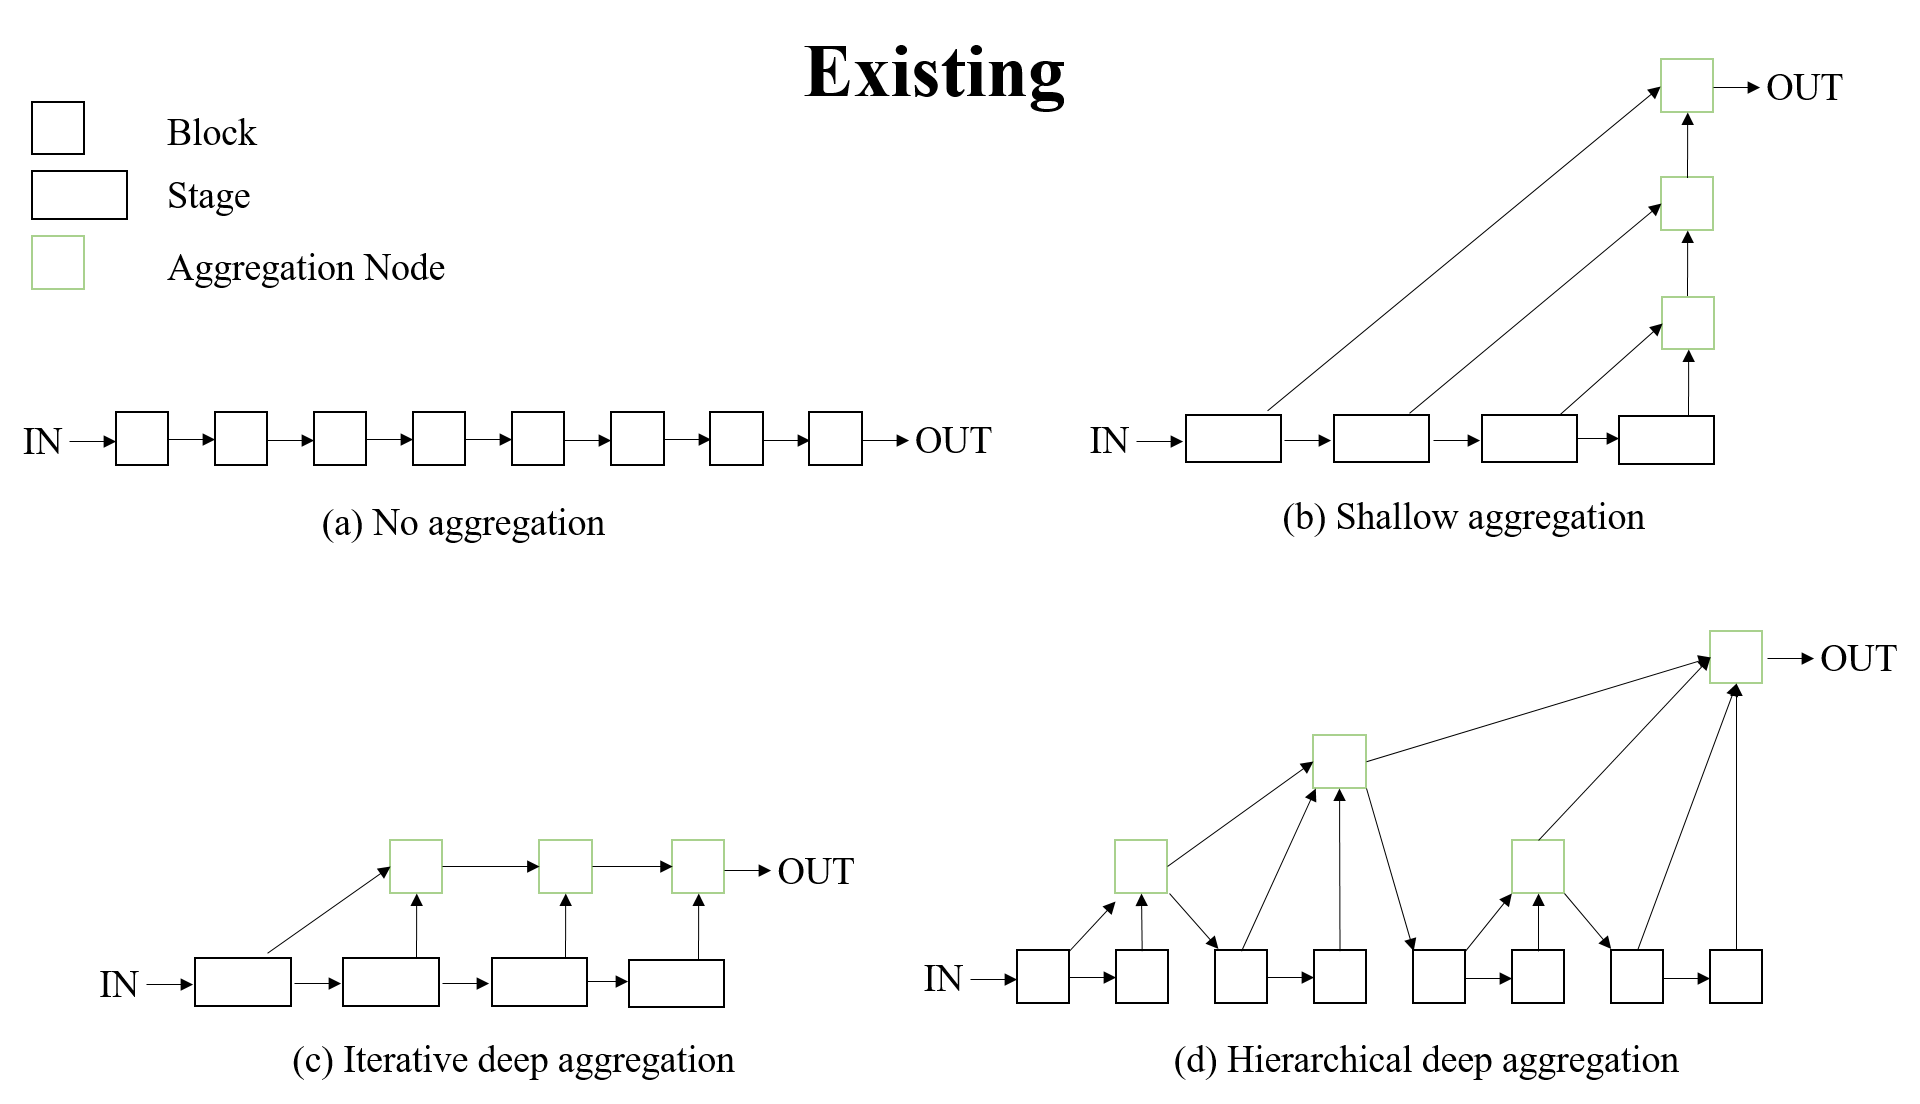
\includegraphics[width=12cm]{Figures/existed_aggr.png}
	\caption{Different approaches to aggregation. (a) composes blocks without aggregation as is the default for classification and regression networks. (b) combines parts of the network with skip connections, as is commonly used for tasks like segmentation and detection, but does so only shallowly by merging earlier parts in a single step each. }
	\label{fig:exited_aggr}
\end{figure}
Existing work on convolutional layer aggregation focus on the linear and non-linear combination of different layers. Fig.~\ref{fig:exited_aggr}(b) show the shallowest aggregation, which simply make linear combination on all blocks. Yu[] proposed iterative deep aggregation (IDA) and hierarchical deep aggregation (HDA) as shown in Fig.~\ref{fig:exited_aggr}(c) and Fig.~\ref{fig:exited_aggr}(d).  IDA iterativly merges lower layers with deeper layers to refine shallow features. HDA employs deep and branching structure to better preserve features.

Recurrent aggregation using LSTM (RA-LSTM) merges blocks as a sequence to both contain the spatial and channel-wise information and explore the transformation relationship according to the order. The mapped feature vectors share the same length and form a regular sequence. One typical sequential data is text, and RNN has shown their tremendous advantage on processing text data. The successful application of RNNs mainly rely on their memory on contextual information. The memory mechanism helps combine all the input inforamtion together and is capable of detecting the correlation among all steps. LSTM employs input gate, forget gate and output gate to realize the long short-term memory, which naturally introduce attention mechanism to focus on useful information. LSTM takes input of $n$ steps, with all the input vector sharing the same dimention and the mapped feature matrix $V\in \mathbb{R}^{N\times C}$ satisfies the requirements. The output vector of LSTM $U$ can be calculated by:
\begin{equation}
U = F_{LSTM}(V)
\end{equation}
where $F_{LSTM}$ denote a standard LSTM structure with forget gates.The inputs of LSTM connect to the convolutional blocks through mapping nodes, and the gradient can be directly back propagated to all the blocks. These connections contribute to avoiding vanishing gradient problem and helps convolutional blocks to extract more expressive sequential features.

The output vector $U$ of LSTM contains squeezed and abstract information through the convolutional network. To utilize this abstract feature, we embed a simple non-linear combination before the output layer as:
\begin{equation}
u = \sigma(WU)
\end{equation}
where $\sigma$ denote the ReLU[] function. 

\subsection{Exemplars: VGG-RA and ResNet-RA}
The flexibility of recurrent aggregation using LSTM means that it can be directly appended to standard convolutional neural networks, without any modification on the original structure. Given a normal CNN, all we need to do is selecting output features to be employed, mapping them to vectors with the same length and arrange them into a matrix as the input of LSTM. In this paper, we apply RA-LSTM to modern architexctures VGGNet[] and ResNet[] to show the efficiency.

For non-blocked networks such as VGGNet, feature selection need to be done before layer aggregation. In general, modern CNN architectures repeat serval convolution followed by a down-sampling operation to extract features. We classify the convolutional layers sharing the same feature resolution into the same stage, and split each stage into 1 or more blocks manually. Then the network is grouped into blocks with each blocks contains more than one convolutional layers. We construct VGG-RA network by simply choose the first three stages of VGGNet and aggregrate it with a LSTM network. The VGG-RA network structure is shown in Fig.~\ref{fig:VGG-RA}.
\begin{figure}  
	\centering
	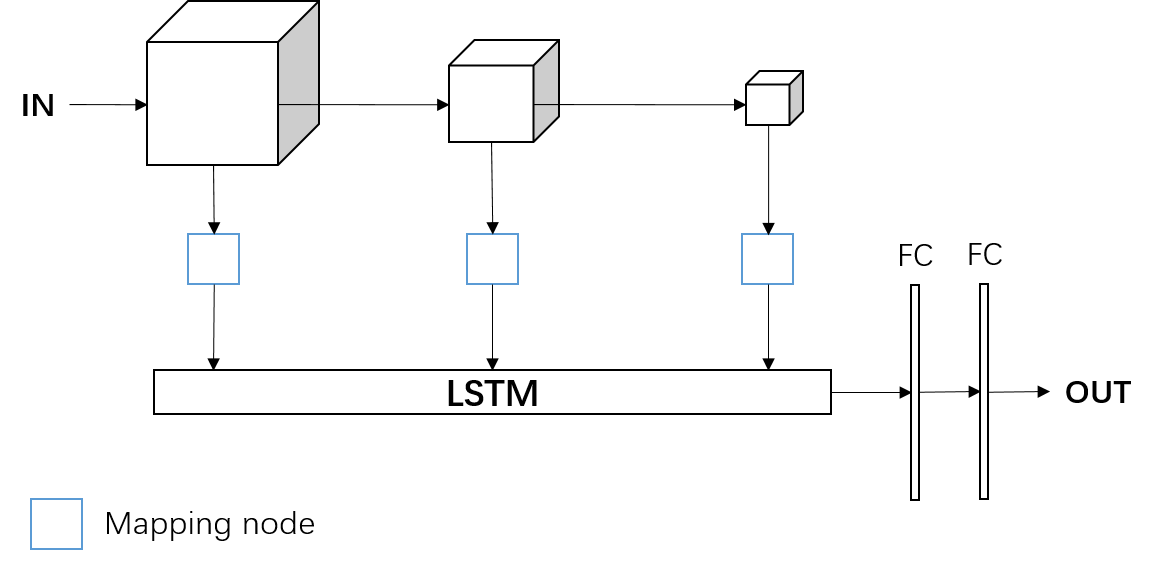
\includegraphics[width=12cm]{Figures/CNN-RA.png}
	\caption{Structure of CNN-RA}
	\label{fig:VGG-RA}
\end{figure}

Blocked networks like ResNet are easy to apply RA-LSTM, with each block output a feature matrix. For complex blocks such as a residual block with 20 or more convolutional layers, we can also split them into more subblocks. We employ ResNet with 3 residual blocks to build ResNet-RA, and the structure diagram is shown in Fig.~\ref{fig:ResNet-RA}.
\begin{figure}  
	\centering
	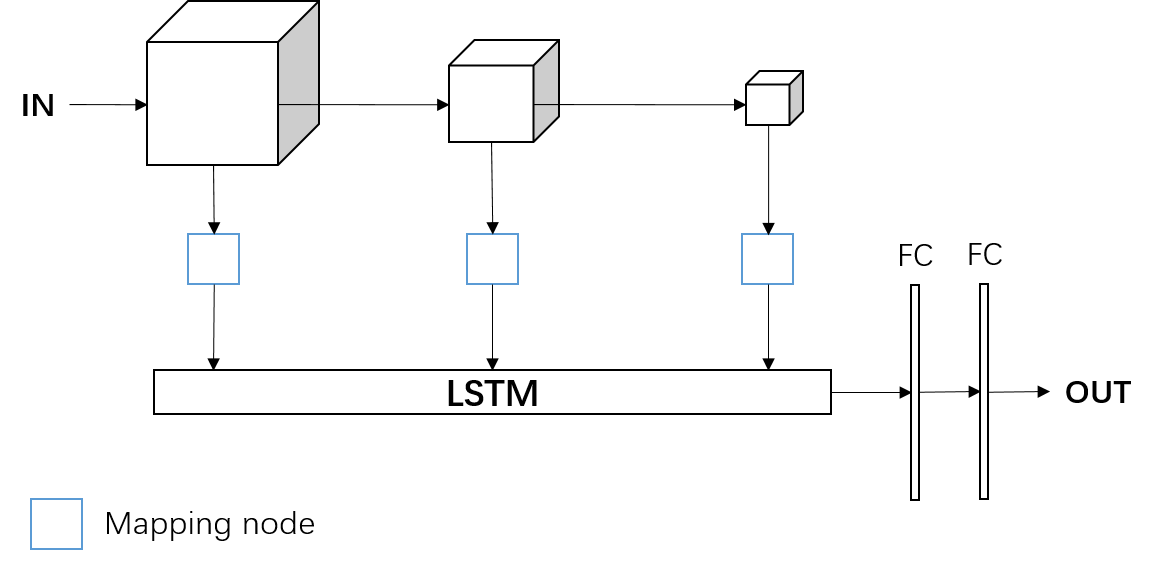
\includegraphics[width=12cm]{Figures/CNN-RA.png}
	\caption{Structure of CNN-RA}
	\label{fig:ResNet-RA}
\end{figure}

\section{Training Details}
\subsection{Feature selection}
Given a standard CNN structure, we just select some of the convolutional layers to be aggregrated. A large number of outputs brings with complexity and much redundant information, which makes against the appearance and convergence rate of LSTM. The selected blocks has to satisfies three rules we proposed: (a)each block contain at least 2 convolutional layers, (b)each stage contains at most 2 blocks, (c)the selected layer in each stage should be located before the corresponding down-sampling layer. According to these three rules, we split VGGNet and ResNet into 3 blocks, which is shown in Table~\ref{table:headings}.
\subsection{Feature Mapping}

Feature mapping nodes transform the feature matrix of CNN layers to the input ventors of LSTM. The feature resolution and channel number varies from shallow layers to deep layers, however, LSTM requires inputs of a common dimension. We first take global average pooling on the last block output and generate a standard vector. In general, previous blocks hold larger feature map and fewer channels. We propose to treat differnet blocks according to their feature resolutions, and group them into three levels, shallow level, mid level and last level. The last level only contains the final block. The mid level contains blocks whose feature resolutions is $2\times$ or $1\times$ larger than the final blocks. The shallow blocks contains the rest blocks. 

The last block outputs a standard vector $v_e$ with the same dimention as the last channel number $C$ by global average pooling. For mid level blocks, we employ a single convolutional layer with to transform the feature resolution and channel number into the same as the final block and then take the global average pooling operation. Blocks in shallow levels are handled specially, because their feature resolutions are at least $4\times$ larger than the final block and the receptive fields may not cover the input size. These blocks contains more details information which we hope to utilize. Thus we first combine the spacial information by a convolutional layer with stride 2, and take average pooling with the kernel size equal to the shape of the final block. A feature matrix $u \in \mathbb{R}^{h\times w \times c}$ is then generated with $h\times w \times c = C$ and is expanded to $v_s$. All feature vectors are arranged into a matrix $V$ as the input of LSTM.

\subsection{Implementation Details}

We verify the effectiveness of RA-LSTM on three famous classification benchmark Cifar10[], SVHN[] and Cifar100[]. All these three datasets contain images with size $32\times 32\times 3$. We do data augmentation on Cifar10 and Cifar100 by first resizing the images to $40\times 40\times 3$ and then randomly cropped them to $32\times 32\times 3$. We also flip the images at random.

Considering the small resolution of images, we do some manipulation on the original network structure. Standard VGGNet consists of five down-sampling layers and cannot be directly applied to small images. We select the first three stages with each containing two convolutional layers and a pooling layer, which we denote as VGG-1 in this paper. The selected network contains totally 6 convolutional layers and we group them into 3 blocks with each containing 2 layers. VGG-1 is shallow and each stage contains only two layers. We then double each block to 4 layers and generate a new network denoted as VGG-2. VGG-2 contains 12 layers and is also grouped into 3 blocks according to their feature resolutions. ResNet is block-wise and we assemble three blocks with each containg 20 convolutional layers. To eliminate the influence of complexity by applying LSTM, we embed a fully-connected layers before output layer in the re-implementation.

We apply RA-LSTM to the three networks by appending a normal LSTM structure. The aggregrated network is then correspondingly denoted as VGG-1-RA, VGG-2-RA and ResNet-RA. The structure parameters is list in Table~\ref{table:struc}. We employ Batch-Normalization in each model to accelerate the convergence, and learning rate decay to optimize the convergence results.

\setlength{\tabcolsep}{4pt}
\begin{table}
\begin{center}
\caption{
Network parameters of network re-implementation and aggregation.
}
\label{table:struc}
\begin{tabular}{lllll}
\hline\noalign{\smallskip}
Network& Block1 & Block2 & Block3 & Classifier\\
\noalign{\smallskip}
\hline
\noalign{\smallskip}
\hline
\end{tabular}
\end{center}
\end{table}
\setlength{\tabcolsep}{1.4pt}


\section{Results}

\subsection{Classification with RA-LSTM}

We evaluate our recurrent aggregation methods on three image classification benchmark datasets Cifar10, SVHN and Cifar100 using three standard networks. We first re-implement VGG-1, VGG-2 and ResNet shown in Table~\ref{table:struc}, and train them on the three datasets. The networks are trained by SGD with momentum 0.9. We set weight decay as $10^{-4}$ and batch size as 64. For all the three datasets, we train 100 epoachs. For Cifar10 and SVHN, the learning rates starts at 0.01, and is reduced by 10 at $50_{th}$ and $75_{th}$ epoach. For Cifar100, the learning rates starts at 0.005 and is reduced at $80_{th}$ epoach. The data augmentation is operated on Cifar10 and Cifar100 with random-cropping and flipping. Then we evaluate the trained model on the three test set and take the results as the baselines and are shown in Table~\ref{table:test}.

After the training and evaluation of the re-implemented network, we build VGG-1-RA, VGG-2-RA and ResNet-RA by joining LSTM and the original network with mapping nodes. To be fair, we train the aggregrated network with the same procedure and hyper-parameters.We evaluate our aggregrated network on the three test sets, and the results are shown in Table~\ref{table:test}.
\setlength{\tabcolsep}{4pt}
\begin{table}
\begin{center}
\caption{Validation accuracies on three datasets. The number in parenthesis represents the improvements of network with RA-LSTM over the original network.}
\label{table:test}
\begin{tabular}{l|lll}
\hline\noalign{\smallskip}
Network& Cifar10 & SVHN & Cifar100\\
\noalign{\smallskip}
\hline
\noalign{\smallskip}
VGG-1 & 93.73 & 97.97 & 73.01\\
VGG-1-RA & 94.49(0.76)$\quad$ & 98.11(0.14)$\quad$ & 74.81(1.80)\\
VGG-2 & 94.91 & 98.14 & 76.15\\
VGG-2-RA & 95.30(0.39) & 98.32(0.18) & 77.48(1.33)\\
ResNet & 93.74 & 98.00 & 75.87\\
ResNet-RA & 94.78(\textbf{1.04}) & 98.19(\textbf{0.19}) & 77.85(\textbf{1.98})\\
\hline
\end{tabular}
\end{center}
\end{table}
\setlength{\tabcolsep}{1.4pt}

In Table~\ref{table:test}, the digits represents the improvement on testing accuracy of networks with RA-LSTM over the original ones. For all three networks over the three benchmark datasets, our proposed recurrent aggregation method makes improvements. On Cifar10, ResNet-RA achieves over 1\% on testing accuracy. On Cifar100, all the three networks with RA-LSTM achieves more than 1\% improvements, and ResNet-RA even increase remarkably 1.98\%.

These comparsion experiments show the effectiveness of RA-LSTM. Considering the complexity and difficulty of the datasets themselves, Cifar100 contains 100 classes while Cifar10 and SVHN contains 10. The otherness of intra-class images in Cifar10 is much larger SVHN. Thus we rank them as Cifar100, Cifar10 and SVHN according to their complexity. The testing results show that, all these three networks show better performance on simple datasets over the complex one, and networks with RA-LSTM show the same phenomenon. Paying attention to the improvements on the three datasets and we notice that, the increment of accuracy of three networks is larger when the task is more complex. The improvement on SVHN is less than 0.2\%, and that of Cifar10 achieves 1.04\%, while the accuracy increases up to 1.98\% over Cifar100. The difference of testing results is caused by two reasons. The first is these networks are capable to deal with simple tasks well, and the upside potential is relatively smaller than the comple tasks. the second reason is concluded as the effectiveness of infomation aggregation. For simple tasks such as SVHN classification, high-level features are enough to distinguish different classes. However, for complex problems like Cifar100, the intra-class information is complicated with backgrounds and a variety samples of the same class. Then we need to utilize the features from low-level to high-level and their combination patterns. The results indicated that the recurrent aggrement methods works better on more complex tasks. Another remarkable fact is that, the RA-LSTM shows better results on ResNet which has totally 61 layers. In ResNet, each block contains 20 convolutional layers, which brings significant difference between two blocks. RA-LSTM seems to work better on capturing feature transformation relationship of deeper blocks.

Our model takes different learning decay between Cifar10, SVHN and Cifar100. In Fig.~\ref{fig:Cifar10} and Fig.~\ref{fig:Cifar100} we show the training procedure on Cifar10 and Cifar100. It can be seen that, on Cifar10, recurrent aggregation methods helps the network converge faster and show better final results. On Cifar100, all the three networks converges slower at the beginning with RA-LSTM, however, they achieve higher performance after learning rate decay. ResNet-RA increase the most at the learning rate decay point, and surpass VGG-2-RA at the end. These learning curves how the different effect of RA-LSTM on various tasks. For simple tasks, networks with aggregation converges faster and achieve better results in the end. For complex tasks, recurrent aggregation brings with lower convergence but higher accuracy eventually. The appended LSTM help extract more expressive features, and it takes longer to better fit the complex dataset.
\begin{figure}   
	\centering
	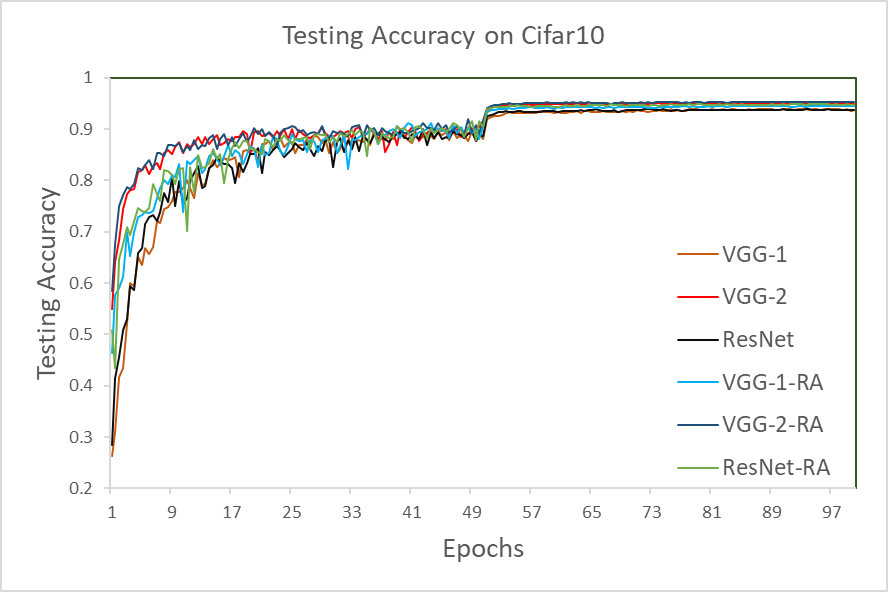
\includegraphics[width=10cm]{Figures/Cifar10.png}
	\caption{Structure of CNN-RA}
	\label{fig:Cifar10}
\end{figure}
\begin{figure}  
	\centering
	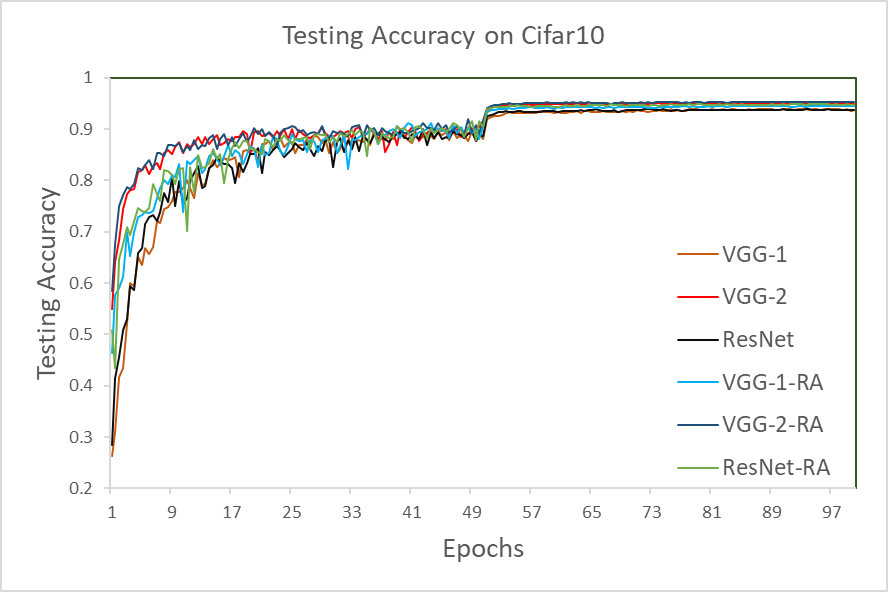
\includegraphics[width=8cm]{Figures/Cifar10.png}
	\caption{Structure of CNN-RA}
	\label{fig:Cifar100}
\end{figure}

\subsection{More Explorations}
To better understand the effectiveness of our proposed RA-LSTM, we explore some other methods to employ the outputs of LSTM. 

\section{Conclusion}

\section{Paper formatting}

\subsection{Language}

All manuscripts must be in English.

%------------------------------------------------------------------------- 
\subsection{Paper Length}
The submission page length is 14 pages for content plus maximum two pages for references.
%This brings the {\em maximum} length for submission to 14 pages. 
Over-length papers will
simply not be reviewed. This includes papers where the margins and
formatting are deemed to have been significantly altered from those
laid down by this style guide. The reason such papers will not be
reviewed is that there is no provision for supervised revisions of
manuscripts. 

%------------------------------------------------------------------------- 
\subsection{Paper ID}

It is imperative that the paper ID is mentioned on each page of the manuscript.
The paper ID is a number automatically assigned to your submission when 
registering your paper submission on CMT.

%------------------------------------------------------------------------- 
\subsection{Dual Submission}

By submitting a manuscript to ACCV 2018, the author(s) assert that it has
not been previously published in substantially similar
form. Furthermore, no paper which contains significant overlap with
the contributions of this paper either has been or will be submitted
during the ACCV 2018 review period to either a journal or a
conference. However, the manuscript may also be submitted to
one workshop that is accompanying ACCV 2018.

If there are any papers that may appear to the reviewers to violate
this condition, then it is your responsibility to (1) cite these
papers (preserving anonymity as described in Section~\ref{sec:blind}
of this example paper, (2) argue in the body of your paper why your
ACCV paper is non-trivially different from these concurrent
submissions, and (3) include anonymized versions of those papers in
the supplemental material.

%------------------------------------------------------------------------- 
\subsection{Supplemental Material} 

Authors may optionally upload supplemental material. Typically, this
material might include videos of results that cannot be included in
the main paper, anonymized related submissions to other conferences
and journals, and appendices or technical reports containing extended
proofs and mathematical derivations that are not essential for
understanding of the paper. Note that the contents of the supplemental
material should be referred to appropriately in the paper and that
reviewers are not obliged to look at it.

All supplemental material must be zipped or tarred into a single file. There is a 30~MB limit on the size of this file. The deadline for supplemental material is a week after the main paper deadline.

%------------------------------------------------------------------------- 
\subsection{Line Numbering}

All lines should be numbered, as in this example document. This makes
reviewing more efficient, because reviewers can refer to a line on a
page. If you are preparing a document using a non-\LaTeX\
document preparation system, please arrange for an equivalent line numbering. Note that accepted papers need to be submitted as a \LaTeX\
document in the style as defined in this document.

%------------------------------------------------------------------------- 
\subsection{Mathematics}

Please number all of your sections and displayed equations.  Again,
this makes reviewing more efficient, because reviewers can refer to a
line on a page.  Also, it is important for readers to be able to refer
to any particular equation.  Just because you did not refer to it in
the text does not mean some future reader might not need to refer to
it.  It is cumbersome to have to use circumlocutions like ``the
equation second from the top of page 3 column 1.''  (Note that the
line numbering will not be present in the final copy, so is not an
alternative to equation numbers).  Some authors might benefit from
reading Mermin's description of how to write mathematics:
\url{http://www.pamitc.org/documents/mermin.pdf}.

%===========================================================
\section{Blind Review}
\label{sec:blind}

Many authors misunderstand the concept of anonymizing for blind
review.  Blind review does not mean that one must remove
citations to one's own work---in fact it is often impossible to
review a paper unless the previous citations are known and
available.

Blind review means that you do not use the words ``my'' or ``our''
when citing previous work.  That is all.  (But see below for 
techreports).

Saying ``this builds on the work of Lucy Smith [1]'' does not say
that you are Lucy Smith, it says that you are building on her
work.  If you are Smith and Jones, do not say ``as we show in
[7],'' say ``as Smith and Jones show in [7]'' and at the end of the
paper, include Reference~7 as you would any other cited work.

An example of a bad paper:
\begin{quote}
\begin{center}
    {\bf An Analysis of the Frobnicatable Foo Filter}
\end{center}
   
   In this paper we present a performance analysis of our
   previous paper [1], and show it to be inferior to all
   previously known methods.  Why the previous paper was
   accepted without this analysis is beyond me.
   
   [1] Removed for blind review
\end{quote}
   
An example of an excellent paper:   
   
\begin{quote}
\begin{center}
     {\bf An Analysis of the Frobnicatable Foo Filter}
\end{center}
   
   In this paper we present a performance analysis of the
   paper of Smith and Jones [1], and show it to be inferior to
   all previously known methods.  Why the previous paper
   was accepted without this analysis is beyond me.
   
   [1] Smith, L., Jones, C.: The frobnicatable foo
   filter, a fundamental contribution to human knowledge.
   Nature {\bf 381} (2005) 1--213
\end{quote}
   
If you are making a submission to another conference at the same time,
which covers similar or overlapping material, you may need to refer to that
submission in order to explain the differences, just as you would if you
had previously published related work.  In such cases, include the
anonymized parallel submission~\cite{Authors18} as additional material and
cite it as
\begin{quote}
[1]  Authors: The frobnicatable foo filter, ACCV 2018 Submission ID 512,
Supplied as additional material {\tt accv18-512-frfofi.pdf}.
\end{quote}

Finally, you may feel you need to tell the reader that more details can be found elsewhere, and refer them to a technical report.  For conference submissions, the paper must stand on its own, and not {\em require} the reviewer to go to a techreport for further details.  Thus, you may say in the body of the paper ``further details may be found in~\cite{Authors18b}.''  Then submit the anonymized techreport as additional material. Again, you may not assume the reviewers will read this material.

Sometimes your paper is about a problem which you tested using a tool which
is widely known to be restricted to a single institution.  For example,
let us say it is 1969, you have solved a key problem on the Apollo lander,
and you believe that the ACCV audience would like to hear about your
solution.  The work is a development of your celebrated 1968 paper entitled
``Zero-g frobnication: How being the only people in the world with access to
the Apollo lander source code makes us a wow at parties,'' by Zeus.

You can handle this paper like any other.  Do not write ``We show how to
improve our previous work [Anonymous, 1968].  This time we tested the
algorithm on a lunar lander [name of lander removed for blind review].''
That would be silly, and would immediately identify the authors. Instead
write the following:
%
\begin{quotation}
\noindent
   We describe a system for zero-g frobnication.  This
   system is new because it handles the following cases:
   A, B.  Previous systems [Zeus et al. 1968] did not
   handle case B properly.  Ours handles it by including
   a foo term in the bar integral.

   The proposed system was integrated with the Apollo
   lunar lander, and went all the way to the moon.  
\end{quotation}
%
As you can see, the above text follows standard scientific convention,
reads better than the first version, and does not explicitly name you as
the authors.  A reviewer might think it likely that the new paper was
written by Zeus, but cannot make any decision based on that guess.
He or she would have to be sure that no other authors could have been
contracted to solve problem B. \\

\noindent FAQ: Are acknowledgements OK?  -- Answer: No. Please {\it omit
acknowledgements} in your review copy; they can go in the final copy.

%===========================================================
\section{Manuscript Preparation}

This is an edited version of Springer LNCS instructions adapted for
ACCV 2018 full paper submission. 

You will have to use \LaTeX2$_\varepsilon$ for the
preparation of your final (accepted)
camera-ready manuscript together with the corresponding Springer
class file \verb+llncs.cls+.

We would like to stress that the class/style files and the template
should not be manipulated and that the guidelines regarding font sizes
and format should be adhered to. This is to ensure that the end product
is as homogeneous as possible.

%------------------------------------------------------------------------- 
\subsection{Printing Area}

The printing area is $122  \; \mbox{mm} \times 193 \;
\mbox{mm}$.
The text should be justified to occupy the full line width,
so that the right margin is not ragged, with words hyphenated as
appropriate. Please fill pages so that the length of the text
is no less than 180~mm.

%------------------------------------------------------------------------- 
\subsection{Layout, Typeface, Font Sizes, and Numbering}

Use 10-point type for the name(s) of the author(s) and 9-point type for
the address(es) and the abstract. For the main text, use 10-point
type and single-line spacing.
We recommend using Computer Modern Roman (CM) fonts, Times, or one
of the similar typefaces widely used in photo-typesetting.
(In these typefaces the letters have serifs, {\it i.e.}, short endstrokes at
the head and the foot of letters.)
Italic type may be used to emphasize words in running text. 

{\it Bold type and underlining should be avoided.}

With these sizes, the interline distance should be set so that some 45
lines occur on a full-text page.

%------------------------------------------------------------------------- 
\subsubsection{Headings.}

Headings should be capitalised
({\it i.e.}, nouns, verbs, and all other words
except articles, prepositions, and conjunctions should be set with an
initial capital) and should,
with the exception of the title, be aligned to the left.
Words joined by a hyphen are subject to a special rule. If the first
word can stand alone, the second word should be capitalised.
The font sizes
are given in Table~\ref{table:headings}. (Note that vertical lines
are not common table components anymore.)
%
\setlength{\tabcolsep}{4pt}
\begin{table}
\begin{center}
\caption{
Font sizes of headings. Table captions should always be
positioned {\it above} the tables. A table
caption ends with a full stop.
}
\label{table:headings}
\begin{tabular}{lll}
\hline\noalign{\smallskip}
Heading level $\qquad\qquad$& Example & Font size and style\\
\noalign{\smallskip}
\hline
\noalign{\smallskip}
Title (centered)  & {\Large \bf Lecture Notes \dots} $\qquad$& 14 point, bold\\
1st-level heading & {\large \bf 1 Introduction} & 12 point, bold\\
2nd-level heading & {\bf 2.1 Printing Area} & 10 point, bold\\
3rd-level heading & {\bf Headings.} Text follows \dots & 10 point, bold
\\
4th-level heading & {\it Remark.} Text follows \dots & 10 point,
italic\\
\hline
\end{tabular}
\end{center}
\end{table}
\setlength{\tabcolsep}{1.4pt}

Here are
some examples of headings: ``Criteria to Disprove Context-Freeness of
Collage Languages,'' ``On Correcting the Intrusion of Tracing
Non-deterministic Programs by Software,'' ``A User-Friendly and
Extendable Data Distribution System,'' ``Multi-flip Networks:
Parallelizing GenSAT,'' ``Self-determinations of Man.''

%------------------------------------------------------------------------- 
\subsubsection{Lemmas, Propositions, and Theorems.}

The numbers accorded to lemmas, propositions, theorems, and so forth should
appear in consecutive order, starting with the number one, and not, for
example, with the number eleven.

%------------------------------------------------------------------------- 
\subsection{Figures and Photographs}
\label{sect:figures}

Please produce your figures electronically and integrate
them into your text file. For \LaTeX\ users we recommend using package
\verb+graphicx+ or the style files \verb+psfig+ or \verb+epsf+.

Check that in line drawings, lines are not
interrupted and have constant width. Grids and details within the
figures must be clearly readable and may not be written one on top of
the other. Line drawings should have a resolution of at least 800 dpi
(preferably 1200 dpi).
For digital halftones 300 dpi is usually sufficient.
The lettering in figures should have a height of 2~mm (10-point type).
Figures should be scaled up or down accordingly.
Please do not use any absolute coordinates in figures.

Figures should be numbered and should have a caption which should
always be positioned {\it under} the figures, in contrast to the caption
belonging to a table, which should always appear {\it above} the table.
Please center the captions between the margins and set them in
9-point type
(Fig.~\ref{fig:example} shows an example).
The distance between text and figure should be about 8~mm, the
distance between figure and caption about 5~mm.
\begin{figure}
	\centering
	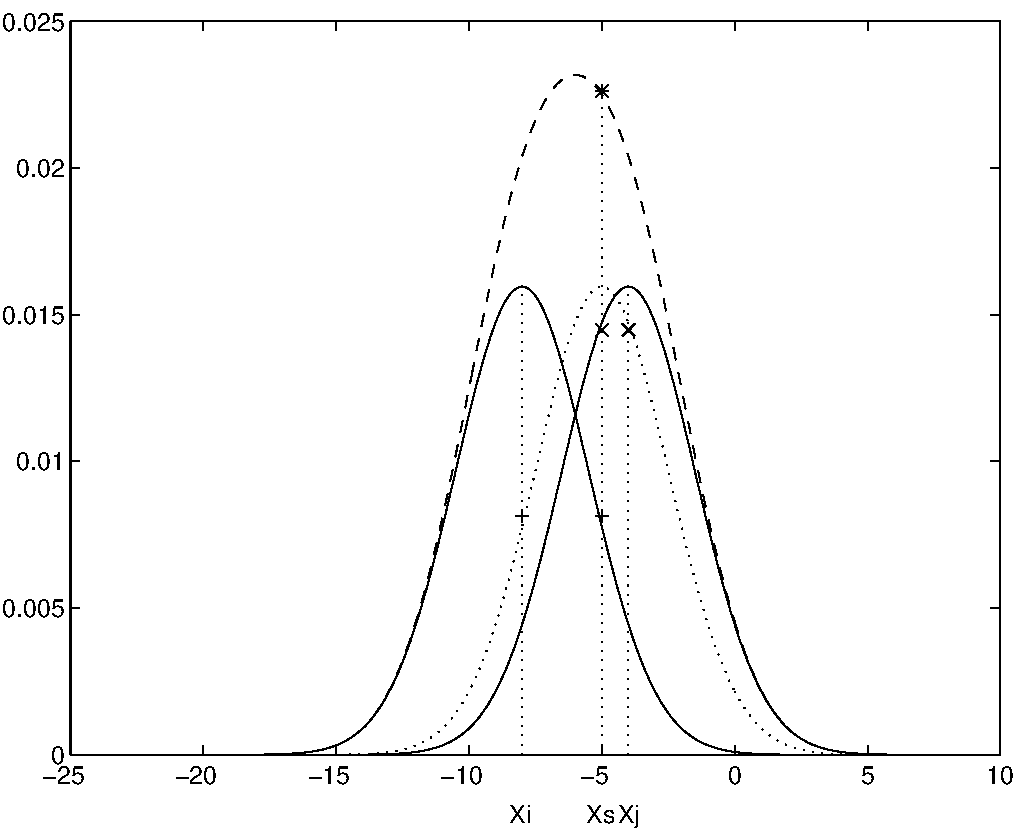
\includegraphics[height=6.5cm]{eijkel2}
	\caption{One kernel at $x_s$ ({\it dotted kernel}) or two kernels at
		$x_i$ and $x_j$ ({\it left and right}) lead to the same summed estimate
		at $x_s$. This shows a figure consisting of different types of
		lines. Elements of the figure described in the caption should be set in
		italics,
		in parentheses, as shown in this sample caption. The last
		sentence of a figure caption should generally end without a full stop}
	\label{fig:example}
\end{figure}

If possible (e.g. if you use \LaTeX) please define figures as floating
objects. \LaTeX\ users, please avoid using the location
parameter ``h'' for ``here''. If you have to insert a pagebreak before a
figure, please ensure that the previous page is completely filled.

%------------------------------------------------------------------------- 
\subsection{Formulas}

Displayed equations or formulas are centered and set on a separate
line (with an extra line or halfline space above and below). Displayed
expressions should be numbered for reference. The numbers should be
consecutive within each section or within the contribution,
with numbers enclosed in parentheses and set on the right margin.
For example,
%
\begin{equation}
  \psi (u) = \int_{o}^{T} \left[\frac{1}{2}
  \left(\Lambda_{o}^{-1} u,u\right) + N^{\ast} (-u)\right] \mathrm{d}t~.
  \label{equ:dt}
\end{equation}

Please punctuate a displayed equation in the same way as ordinary
text but with a small space before the end punctuation.

%Do not punctuate a displayed equation in the same way as ordinary
%text; for example, there is no full stop at the end of Equ.~(\ref{equ:dt}).

%-------------------------------------------------------------------------
\subsection{Program Code}

Program listings or program commands in the text are normally set in
typewriter font, for example, CMTT10 or Courier.

\medskip

\noindent
{\it Example of a Computer Program}
\begin{verbatim}
program Inflation (Output)
  {Assuming annual inflation rates of 7%, 8%, and 10%,...
   years};
   const
     MaxYears = 10;
   var
     Year: 0..MaxYears;
     Factor1, Factor2, Factor3: Real;
   begin
     Year := 0;
     Factor1 := 1.0; Factor2 := 1.0; Factor3 := 1.0;
     WriteLn('Year  7% 8% 10%'); WriteLn;
     repeat
       Year := Year + 1;
       Factor1 := Factor1 * 1.07;
       Factor2 := Factor2 * 1.08;
       Factor3 := Factor3 * 1.10;
       WriteLn(Year:5,Factor1:7:3,Factor2:7:3,Factor3:7:3)
     until Year = MaxYears
end.
\end{verbatim}
%
\noindent
{\small (Example from Jensen K., Wirth N. (1991) Pascal user manual and
report. Springer, New York)}

%------------------------------------------------------------------------- 
\subsection{Footnotes}

The superscript numeral used to refer to a footnote appears in the text
either directly after the word to be discussed or, in relation to a
phrase or a sentence, following the punctuation sign (comma,
semicolon, or full stop). Footnotes should appear at the bottom of
the
normal text area, with a line of about 2~cm in \TeX\ and about 5~cm in
Word set
immediately above them.\footnote{The footnote numeral is set flush left
	and the text follows with the usual word spacing. Second and subsequent
	lines are indented. Footnotes should end with a full stop.}

%------------------------------------------------------------------------- 
\subsection{Citations}

The list of references is headed ``References'' and is not assigned a
number in the decimal system of headings. The list should be set in small print and placed at the end of your contribution, in front of the appendix, if one exists.

Please do not insert a page break before the list of references if the page is not completely filled. Citations in the text are with square brackets and consecutive numbers, such as \cite{Alpher02}, or \cite{Alpher03,Herman04}.

%References are listed in alphabetic order by the surname of the first author, or the identifying word (e.g., in case of a website). Have
%all anonymized references at the beginning of the list.

%here would be your acknowledgement (if any) in the final accepted paper

%------------------------------------------------------------------------- 
\section{Conclusions}

The paper ends with a conclusion. 

%===========================================================
\bibliographystyle{splncs}
\bibliography{egbib}

%this would normally be the end of your paper, but you may also have an appendix
%within the given limit of number of pages
\end{document}
